\documentclass[a4paper,12pt,bahasa]{extarticle}
\usepackage[a4paper]{geometry}
\geometry{verbose,tmargin=2cm,bmargin=2cm,lmargin=2cm,rmargin=2cm}

\usepackage{fontspec}
\setmainfont{Calibri}
\setmonofont{Courier 10 Pitch}

\setlength{\parindent}{0cm}

\usepackage{amsmath}

\usepackage{setspace}
\onehalfspacing

\usepackage{xcolor}
\usepackage{float}
\usepackage{graphicx}
\usepackage{hyperref}
\usepackage{url}

\usepackage{float}

\usepackage{minted}
%\newminted{verilog}{breaklines}
\newminted{verilog}{breaklines,fontsize=\small}
\newminted{text}{breaklines,fontsize=\small}

\usepackage{babel}

\definecolor{mintedbg}{rgb}{0.95,0.95,0.95}
\usepackage{mdframed}

%\global\mdfapptodefinestyle{verilognotes}{%
%rightline=true,%
%innerleftmargin=10,%
%innerrightmargin=10,%
%frametitlerule=true,%
%frametitlerulewidth=2pt}

\mdfdefinestyle{verilognotes}{%
  linecolor=blue,
  linewidth=1pt,
  frametitlerule=true,
  frametitlerulewidth=2pt
}

%\BeforeBeginEnvironment{minted}{\begin{mdframed}[backgroundcolor=mintedbg]}
%\AfterEndEnvironment{minted}{\end{mdframed}}


\begin{document}


\title{MODUL V \\
Implementasi Rangkaian Digital dengan FPGA}
\author{}
\date{}
\maketitle

\section{Tujuan}

\section{Alat dan Bahan}


\section{Dasar Teori}

programmable logic devices dan FPGA

Entri desain

\subsection{Pengenalan Quartus Prime}

Quartus Prime merupakan perangkat lunak CAD (computer-assisted design)
yang digunakan untuk desain rangkaian digital. Quartus Prime dikembangkan
oleh Altera. Versi Lite dari Quartus Prime dapat diunduh secara gratis
pada laman Altera\footnote{\url{http://dl.altera.com/?edition=lite}}.
Quartus Prime dapat dijalankan pada
platform Windows dan Linux.
Jendela utama dari Quartus Prime Lite dapat dilihat pada Gambar
\ref{fig:main_window}.

\begin{figure}
\centering
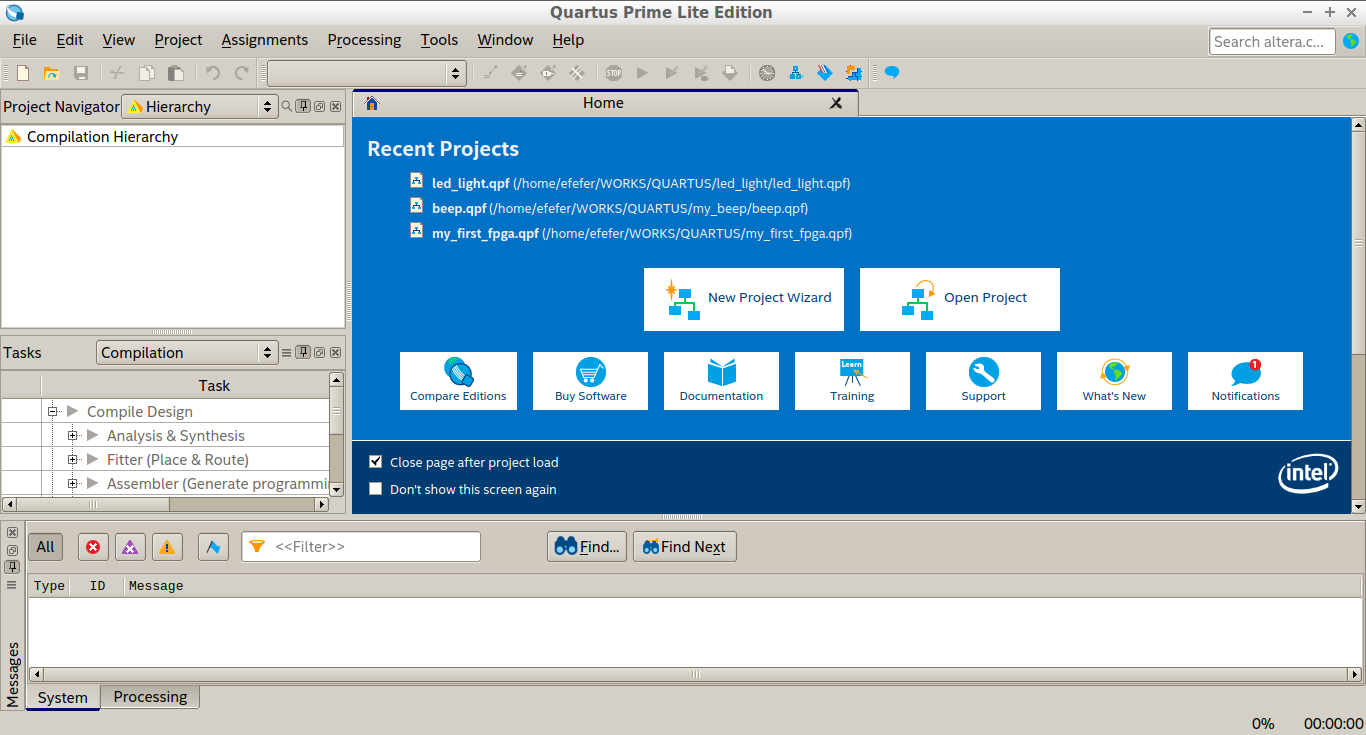
\includegraphics[width=\textwidth]{images/FirstOpen.png}
\par
\caption{Tampilan jendela utama Quartus Prime Lite}\label{fig:main_window}
\end{figure}

Dengan menggunakan CAD, setidaknya ada dua cara untuk
mendesain rangkaian digital:
\begin{itemize}
\item \textit{schematic capture}, dengan membuat skematik dari rangkaian yang
diinginkan.
\item menggunakan Hardware Description Language (HDL).
Dua jenis HDL yang paling populer adalah Verilog dan VHDL.
Kedua bahasa tersebut telah diadopsi sebagai IEEE Standard.
Pada tulisan ini akan digunakan Verilog.
\end{itemize}

Kita akan mulai dengan membuat project baru dan menambahkan skematik.

\subsection{Membuat project baru}
Berikut ini adalah langkah-langkah yang digunakan untuk membuat New Project
pada Quartus Prime Lite.

\framebox[1.1\width]{\textbf{Langkah 1}}
Pilih menu: \textbf{File $\rightarrow$ New Project Wizard}.
Jendela baru seperti pada gambar berikut akan
muncul.
Centang \textbf{Don't show me this introduction again} jika perlu.
Klik \textbf{Next}.
\begin{figure}[H]
\centering
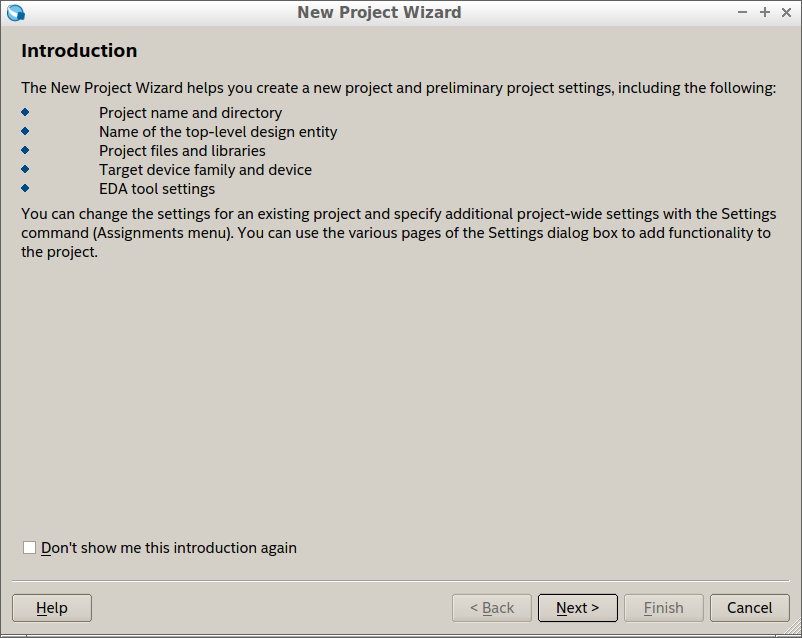
\includegraphics[width=0.5\textwidth]{images/NewProjectWizard_1.png}
\par
\end{figure}


\framebox[1.1\width]{\textbf{Langkah 2}}
Tentukan nama Project yang akan dibuat dan direktori di
mana file-file yang terkait dengan Project ini akan disimpan. Contoh
dapat dilihat pada gambar berikut. Setelah itu, klik \textbf{Next}
setelah semua isian diberikan.

\begin{figure}[H]
\centering
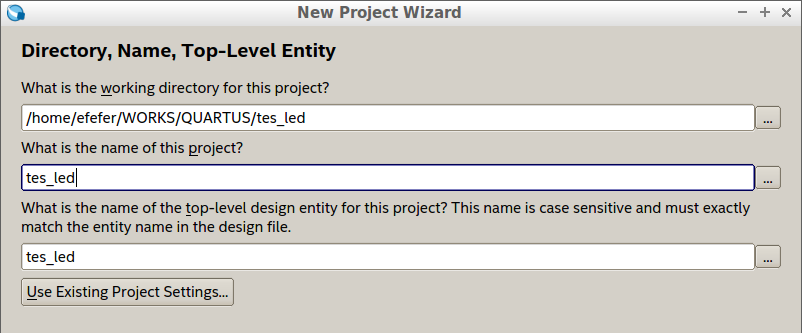
\includegraphics[width=0.5\textwidth]{images/NewProjectWizard_2.png}
\par
\end{figure}


\framebox[1.1\width]{\textbf{Langkah 3}}
Kita diminta untuk memilih jenis Project. Pilih \textbf{Empty Project}.
Setelah itu, klik \textbf{Next}.

\begin{figure}[H]
\centering
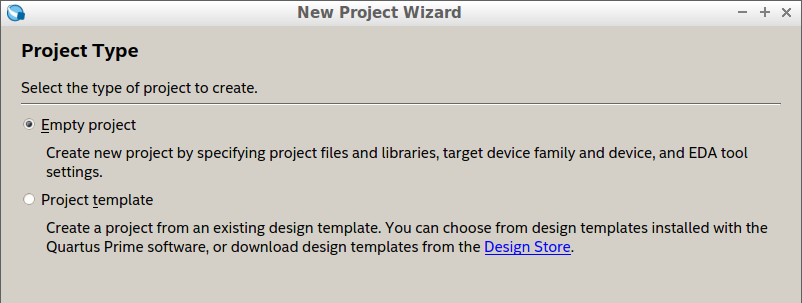
\includegraphics[width=0.5\textwidth]{images/NewProjectWizard_3.png}
\par
\end{figure}


\framebox[1.1\width]{\textbf{Langkah 4}}
Pada langkah ini kita dapat menambahkan file yang sudah ada ke Project
yang akan dibuat. Jika tidak ada langkah ini dapat dilewati.
Klik \textbf{Next}.

\begin{figure}[H]
\centering
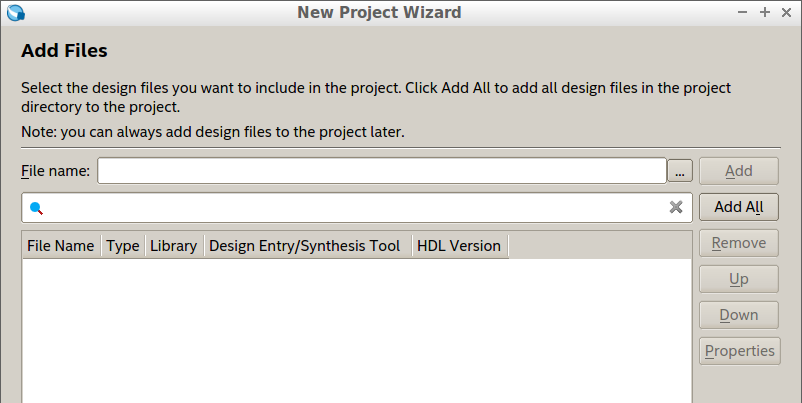
\includegraphics[width=0.5\textwidth]{images/NewProjectWizard_4.png}
\par
\end{figure}

\framebox[1.1\width]{\textbf{Langkah 5}}
Pada langkah ini, kita harus memilih \textbf{Device Family} dan
\textbf{Name}. Untuk \textbf{Device Family} pilih \textbf{Cyclone IV E}.

\begin{figure}[H]
\centering
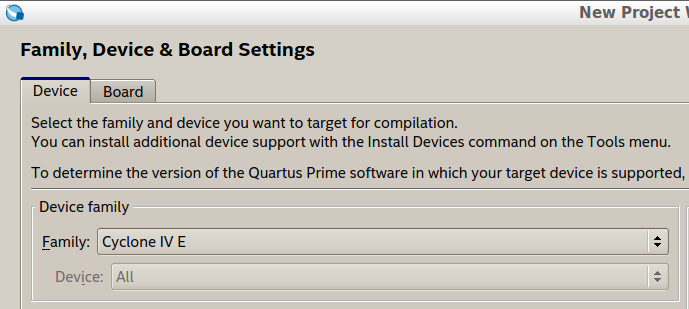
\includegraphics[width=0.5\textwidth]{images/NewProjectWizard_5_device_family.png}
\par
\end{figure}

Pada \textbf{Available Device} pilih \textbf{EP4CE6E22C8}.
Setelah itu, klik \textbf{Next}.

\begin{figure}[H]
\centering
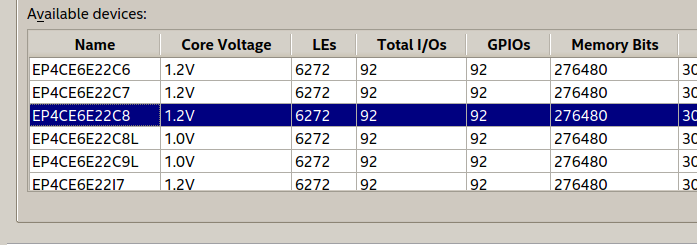
\includegraphics[width=0.5\textwidth]{images/NewProjectWizard_5_device_name.png}
\par
\end{figure}


\framebox[1.1\width]{\textbf{Langkah 6}}
Quartus akan meminta kita untuk memilih setting beberapa tools yang
mungkin digunakan. Untuk sementara pilih \textbf{None} untuk semua tools.
Setelah itu, klik \textbf{Next}.

\begin{figure}[H]
\centering
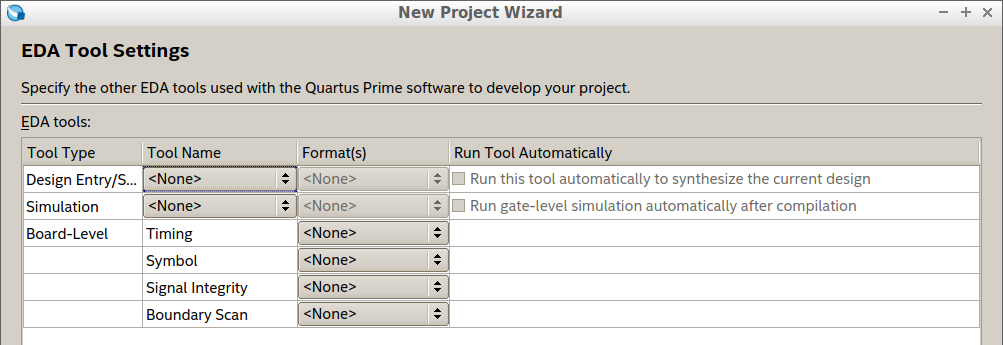
\includegraphics[width=0.5\textwidth]{images/NewProjectWizard_6.png}
\par
\end{figure}

\framebox[1.1\width]{\textbf{Langkah 7}}
Pada bagian akhir, Quartus akan memberikan Summary dari Project yang akan
dibuat. Setelah itu, klik \textbf{Finish}.
\begin{figure}[H]
\centering
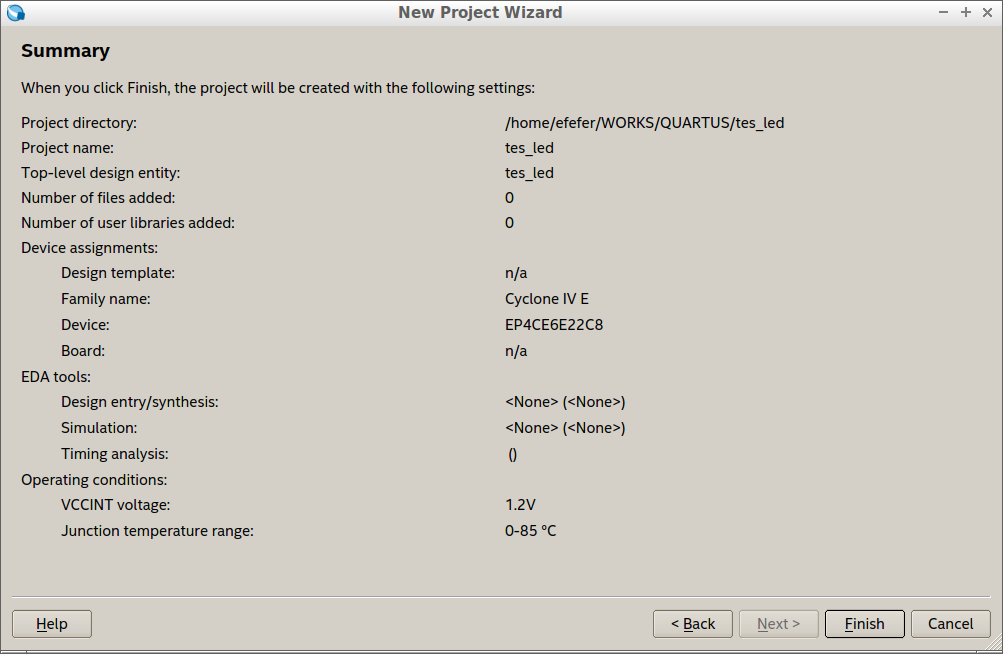
\includegraphics[width=0.5\textwidth]{images/NewProjectWizard_7.png}
\par
\end{figure}




\subsection{Menambahkan skematik baru}\label{subsec:skematik}

Skematik baru dapat ditambahkan ke dalam project dengan memilih menu
\textbf{File $\rightarrow$ New}. Pilih \textbf{New Diagram/Schematic File}, kemudian
\textbf{OK}.

\begin{figure}[H]
\centering
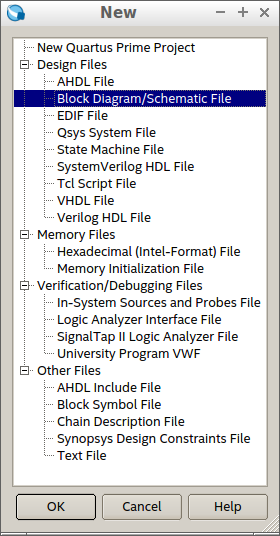
\includegraphics[scale=0.5]{images/NewSchematic.png}
\par
\end{figure}

File skematik kosong akan terbuka pada tab baru dengan nama \textbf{Block1.bdf}.
Kita dapat membuat skematik yang kita inginkan pada file ini.

\begin{figure}[H]
\centering
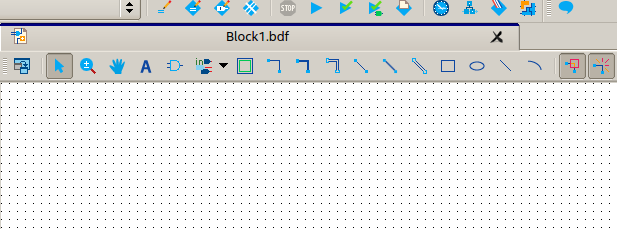
\includegraphics[scale=0.5]{images/EmptySchematic.png}
\par
\end{figure}

Untuk menambahkan komponen, dapat dilakukan dengan cara mengklik toolbar
\textbf{Symbol Tool}.

\begin{figure}[H]
\centering
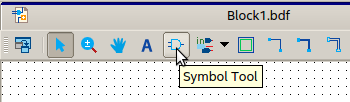
\includegraphics[scale=0.5]{images/SymbolTool.png}
\par
\end{figure}

Komponen yang ingin ditambahkan pada skematik dapat diperoleh dengan
ekspasi node \textbf{Libraries}, mencari komponen tersebut, dan memilihnya.
Misalkan kita ingin menambahkan gerbang AND dengan dua input, maka dapat dipilih
pada \textbf{primitives $\rightarrow$ logic $\rightarrow$ and2}. Klik
\textbf{OK} setelah komponen yang diinginkan telah dipilih.

\begin{figure}[H]
\centering
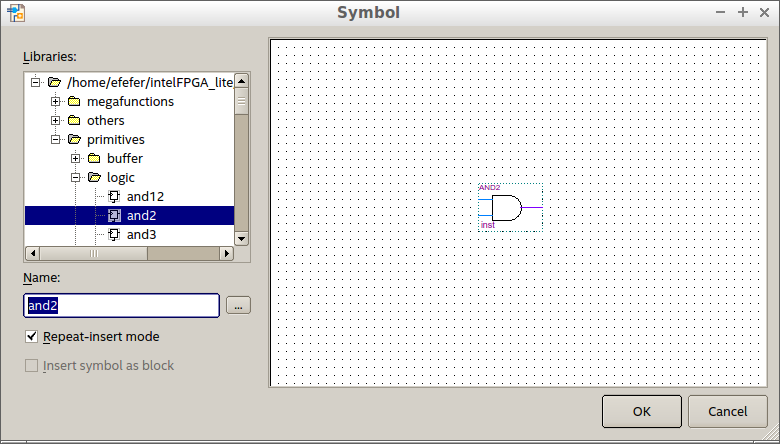
\includegraphics[scale=0.5]{images/BlockAnd.png}
\par
\end{figure}

Pemilihan komponen juga dapat dilakukan dengan mengetikkan nama komponen yang
diinginkan pada isian \textbf{Name}, misalnya \textbf{jkff} untuk J-K flip-flop.

Khusus untuk menambahkan komponen input dan output, dapat juga digunakan
toolbar \textbf{Pin Tool}.
\begin{figure}[H]
\centering
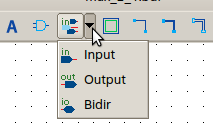
\includegraphics[scale=0.5]{images/PinTool.png}
\par
\end{figure}

Untuk menghubungkan antara satu komponen dengan komponen yang lain, dapat
digunakan \textbf{Orthogonal Node Tool}.
\begin{figure}[H]
\centering
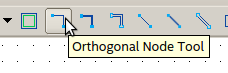
\includegraphics[scale=0.5]{images/OrthogonalNodeTool.png}
\par
\end{figure}

Berikut ini adalah contoh skematik untuk multiplexer 2-to-1:
\begin{figure}[H]
\centering
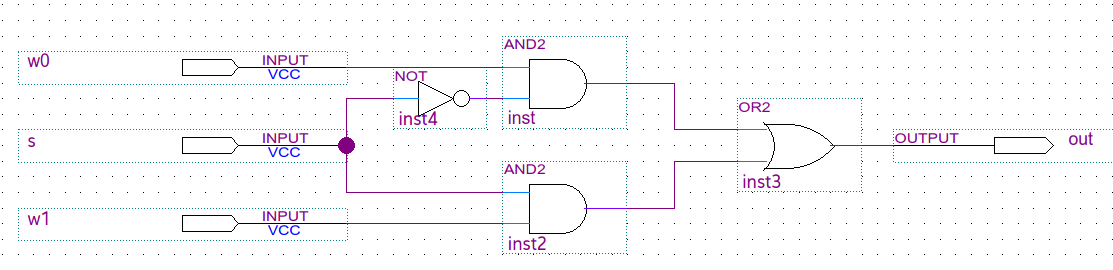
\includegraphics[width=\textwidth]{images/sch_mux_2_1.png}
\par
\end{figure}

Skematik ini kemudian dapat digunakan untuk proses lebih lanjut seperti
simulasi dan download ke hardware FPGA.

Menkonversi ke skematik ke simbol/blok sehingga dapat digunakan sebagai
bagian dari skematik lainnya: gunakan menu \textbf{File $\rightarrow$
Create/Update $\rightarrow$ Create Symbol Files for Current File}.

\begin{figure}[H]
{\centering
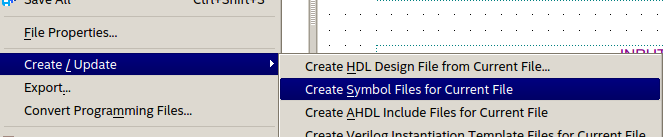
\includegraphics[scale=0.5]{images/MenuCreateSymbol.png}
\par}
\end{figure}

Simbol ini dapat kita gunakan untuk pada skematik lain dengan cara
yang sama ketika kita menambahkan gerbang logika dasar, yaitu dengan
mengklik icon \textbf{Symbol Tool}.

\begin{figure}[H]
{\centering
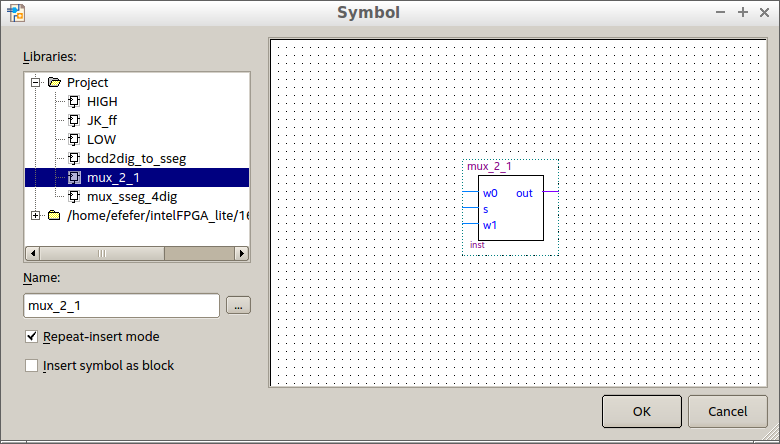
\includegraphics[scale=0.5]{images/symbol_mux_2_1.png}
\par}
\end{figure}

Contoh penggunaan (yang paling sederhana) dapat dilihat pada gambar berikut.

\begin{figure}[H]
{\centering
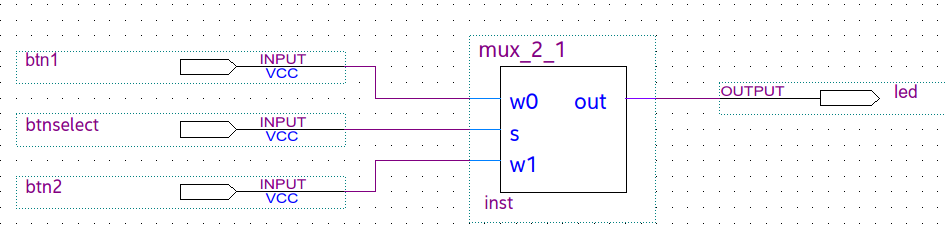
\includegraphics[scale=0.5]{images/tes_mux_2_1.png}
\par}
\end{figure}



\subsection{Bahasa Deskripsi Hardware: Verilog}

Selain menggunakan skematik, desain rangkaian digital juga dapat dilakukan
dengan menggunakan HDL (\textit{hardware description language})
seperti Verilog dan VHDL.
Pada kesempatan kali ini kita akan menggunakan Verilog.

Verilog pada awalnya dikembangkan sebagai alat untuk simulasi serta
verifikasi dari rangkaian digital.
Verilog dikembangkan oleh Gateway Design Automation, yang
sekarang menjadi bagian dari Cadence Design Systems.
Pada awal perkembangannya Verilog merupakan bahasa
proprietary, akan tetapi pada
tahun 1990 Verilog dilepaskan ke
domain publik. Sejak saat itu Verilog menjadi salah satu
bahasa yang populer untuk mendeskripsikan rangkaian digital.
Pada tahun 1995 Verilog diadopsi sebagai IEEE Standard, yaitu standard
1364-1995. Pada tahun 2001, versi terbaru dari Verilog yang dikenal dengan
Verilog 2001 diadopsi menjadi IEEE Standard 1364-2001.

Pada Quartus Prime, file Verilog dapat ditambahkan ke Project
dengan memilih menu \textbf{File $\rightarrow$ New} dan pilih
\textbf{Verilog HDL File}.

\begin{figure}[H]
\centering
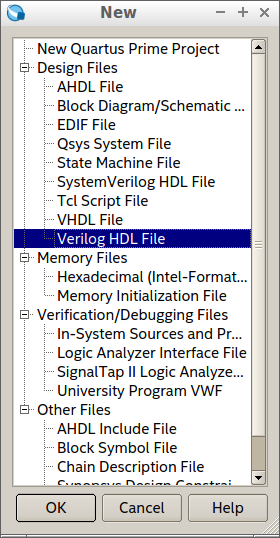
\includegraphics[scale=0.5]{images/new_file_verilog.png}
\par
\caption{New File Verilog HDL}
\end{figure}

File Verilog merupakan file teks sehingga kita dapat menggunakan
teks editor apa saja untuk mengedit file ini.

\subsubsection{Representasi rangkaian digital dengan Verilog}

Terdapat dua pendekatan yang akan kita gunakan untuk mendesain rangkaian
digital dengan Verilog pada praktikum ini
\begin{itemize}

\item struktural: rangkaian digital dideskripsikan dengan struktur
rangkaian tersebut, membangunnya
dengan elemen-elemen rangkaian seperti gerbang logika, dan mendefisinikan
bagaimana elemen-elemen tersebut saling terhubung satu sama lainnya.

\item perilaku (behavioral): rangkaian digital dideskripsikan dengan
perilaku rangkaian tersebut, bukan dengan struktur rangkaiannya secara
langsung. Pendekatan ini dilakukan dengan menggunakan konstruksi
pemrograman Verilog seperti konstruksi \textbf{if}, \textbf{switch}, dan
\textbf{for} yang juga biasa ditemukan pada bahasa
pemrograman komputer. Kompiler Verilog akan melakukan translasi
dari konstruksi pemrograman tersebut menjadi rangkaian digital yang sesuai.z

\end{itemize}


\textbf{Representasi struktural}

Verilog memiliki gerbang logika primitif yang merepresentasikan
gerbang logika yang biasa dipakai pada rangkaian.

Gerbang AND dengan dua input, $x_1$ dan $x_2$,
dan output $y$, misalnya dapat dinyatakan dengan kode Verilog
sebagai berikut.
\begin{verilogcode}
and( y, x1, x2 );
\end{verilogcode}

Gerbang OR dengan 4 input
\begin{verilogcode}
or( y, x1, x2, x3 x4 );
\end{verilogcode}

Inverter $y = \bar{x}$
\begin{verilogcode}
not( y, x );
\end{verilogcode}

Beberapa gerbang primitif pada Verilog dapat diberikan
pada tabel berikut ini.
\begin{table}[h!]
\centering
\begin{tabular}{|ccc|}
\hline
Nama & Deskripsi & Penggunaan \\
\hline\hline
and & $f = (a \cdot b \cdots )$ & \verb|and(f, a, b, ...)| \\
nand & $f = \overline{(a \cdot b \cdots)}$ & \verb|nand(f,a,b,...)| \\
or & $f = (a + b + \cdots)$ & \verb|or(a,b,...)| \\
nor & $f = \overline{(a + b + \cdots)}$ & \verb|nor(a,b,...)| \\
xor & $f = a \oplus b \oplus \cdots $ & \verb|xor(a,b,...)| \\
xnor & $f = a \odot b \odot \cdots $ & \verb|xnor(a,b,...)| \\
not & $f = \bar{a}$ & \verb|not(f,a)| \\
\hline
\end{tabular}
\par
\caption{Beberapa gerbang primitif pada Verilog}
\end{table}

Rangkaian digital yang lebih kompleks
dapat direpresentasikan dengan menggunakan gerbang primitif tersebut.

Dalam tulisan ini, penjelasan mengenai Verilog akan diberikan
melalui contoh.

\begin{figure}[h]
\centering
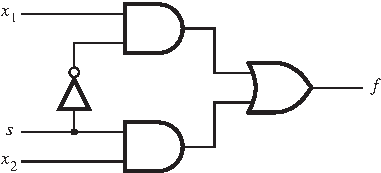
\includegraphics[scale=1.0]{images/fig_2_36.pdf}
\par
\caption{Multiplexer}\label{fig:mux2}
\end{figure}

\framebox[1.1\width]{Contoh 1} Multiplexer pada
Gambar \ref{fig:mux2} dapat dijelaskan dengan kode Verilog berikut.

{\setstretch{1.0}
\begin{verilogcode}
module mux2( x1, x2, s, f );
  input x1, x2, s;
  output f;

  not(k,s);
  and(g,k,x1);
  and(h,s,x2);
  or(f,g,h);
endmodule
\end{verilogcode}
}

Dalam Verilog, rangkaian logika diberikan dalam bentuk modul, didefinisikan
dengan
kata kunci {\tt \textbf{module}}. Suatu modul dapat terdiri dari input dan
output yang disebut sebagai \textit{port}.
Pada contoh di atas, modul dengan nama {\tt \textbf{mux2}} didefinisikan.
Modul {\tt \textbf{mux2}} memiliki 4 port yang bernama {\tt x1}, {\tt x2},
{\tt s}, dan {\tt f}. Pernyataan modul ini diakhiri dengan titik koma.
Pada pernyataan berikutnya, {\tt x1}, {\tt x2} dan {\tt s} dinyatakan
sebagai sinyal input, sedangkan $f$ sebagai sinyal output. Empat baris kode
berikutnya menyatakan struktur dari rangkaian.

Variabel $k$, $g$, dan $h$ tidak dideklarasikan pada kode di atas. Secara default
tipe dari variabel tersebut adalah {\tt wire}.

\framebox[1.1\width]{Contoh 2} Perhatikan rangkaian berikut.

\begin{figure}[H]
\centering
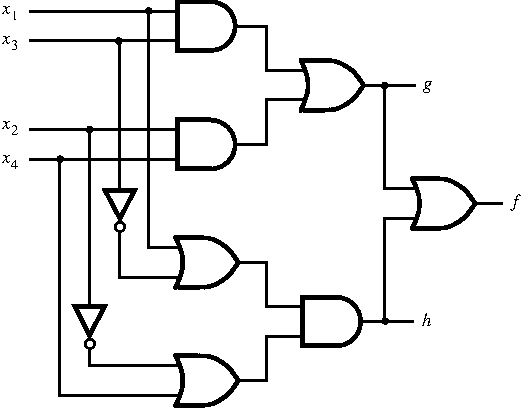
\includegraphics[scale=1.0]{images/fig_2_39.pdf}
\par
\caption{Rangkaian untuk Contoh 2}\label{fig:Contoh2}
\end{figure}

Rangkaian ini memiliki 4 input, yaitu $x_1$, $x_2$, $x_3$, dan
$x_4$, serta 3 output, yaitu $f$, $g$, dan $h$.
Rangkaian ini mengimplementasikan fungsi logika berikut.
\begin{align*}
g & = x_1 x_3 + x_2 x_4 \\
h & = (x_1 + \bar{x_3})(\bar{x_2} + x_4) \\
f & = g + h
\end{align*}

Rangkaian ini dapat diimplementasikan dengan menggunakan kode berikut.
Pada kode ini operator {\tt \textbf{~}} digunakan sebagai pengganti gerbang
NOT.
{\setstretch{1.0}
\begin{verilogcode}
module Contoh2( x1, x2, x3, x4, f, g, h );
  input x1, x2, x3, x4;
  output f, g, h;

  and( z1, x1, x3 );
  and( z2, x2, x4 );
  or( g, z1, z2 );
  or( z3, x1, ~x3 );
  or( z4, ~x2, x4 );
  and( h, z3, z4 );
  or( f, g, h );
endmodule
\end{verilogcode}
}

\textbf{Representasi behavioral}

Menggunakan gerbang logika primitif pada Verilog untuk rangkaian yang
kompleks dapat menjadi tugas yang sulit.
Sebagai alternatif, kita dapat menggunakan ekspresi logika dan
level abtraksi yang lebih tinggi
serta kontruksi pemrograman Verilog untuk mendeskripsikan rangkaian
berdasarkan perilaku dari suatu rangkaian.

Sebagai contoh, output dari multiplexer pada Gambar \ref{fig:mux2}
dapat dijelaskan dengan persamaan logika berikut.
\begin{equation*}
f = \bar{s}x_1 + sx_2
\end{equation*}

Dalam Verilog, persamaan ini dapat dinyatakan dengan kode berikut.
{\setstretch{1.0}
\begin{verilogcode}
module mux2_logic_expr( x1, x3, s, f );
  input x1, x2, s;
  output f;

  assign f = ( ~s & x1 ) | ( s & x2 );
endmodule
\end{verilogcode}
}

Pada kode tersebut, operasi AND dan OR dilakukan dengan menggunakan
operator "{\tt\textbf{\&}}" dan "{\tt\textbf{|}}".

Kata kunci {\tt\textbf{assign}} berarti {\it continuous assignment} untuk
sinyal $f$.
Ketika ada sinyal pada ruas kanan yang berubah, maka $f$ akan dievaluasi ulang.
Jika tidak, maka $f$ akan tetap pada nilai sebelumnya.

Dengan menggunakan ekspresi logika, rangkaian pada Gambar \ref{fig:Contoh2}
dapat dituliskan sebagai berikut.
{\setstretch{1.0}
\begin{verilogcode}
module Contoh2_logic_expr( x1, x2, x3, x4, f, g, h );
  input x1, x2, x3, x4;
  output f, g, h;

  assign g = ( x1 &  x3 ) | (  x2 & x4 );
  assign h = ( x1 | ~x3 ) & ( ~x2 & x4 );
  assign f = g | h;
endmodule
\end{verilogcode}
}

Penggunaan ekspresi logika dapat mempermudah penulisan kode Verilog.
Akan tetapi level abstraksi yang lebih tinggi juga dapat digunakan
dengan cara memberikan spesifikasi mengenai perilaku dari rangkaian.
Rangkaian ini juga dapat dideskripsikan dengan menyatakan perilakunya
sebagai berikut.
\begin{itemize}
\item $f = x_1$ jika $s = 0$, dan
\item $f = x_2$ jika $s = 1$
\end{itemize}

Dalam Verilog, perilaku ini dapat dijelaskan dengan menggunakan
pernyataan {\tt \bf if-else} seperti pada kode berikut.
{\setstretch{1.0}
\begin{verilogcode}
module mux2_behavioral( x1, x2, f );
  input x1;
  input x2;
  output f;

  reg f;

  always @(x1 or x2 or s)
    if( s == 0 )
      f = x1;
    else
      f = x2;
endmodule
\end{verilogcode}
}

Beberapa hal yang perlu diperhatikan terkait kode di atas.

\begin{itemize}
\item Pernyataan {\tt\textbf{if-else}} pada Verilog termasuk dalam
\textit{pernyataan prosedural}.
Verilog mengharuskan pernyataan prosedural diletakkan pada blok
{\tt\textbf{always}},
seperti pada kode di atas. Setiap blok {\tt\textbf{always}} dapat terdiri dari satu
pernyataan, seperti pada contoh di atas, atau beberapa pernyataan prosedural.
Suatu modul Verilog dapat memiliki beberapa
blok {\tt\textbf{always}} yang masing-masing blok tersebut menyatakan suatu bagian
dari rangkaian yang sedang dimodelkan.
\item Pernyataan dalam blok {\tt\textbf{always}} akan dievaluasi sesuai dengan urutan yang
diberikan dalam kode. Hal ini kontras dengan pernyataan
\textit{continuous assignment}
yang dievaluasi secara paralel dan tidak bergantung pada urutan yang diberikan
di kode.
\item Pada blok {\tt\textbf{always}}, setelah simbol \textbf{\@},
dalam tanda kurung, disebut
dengan \textit{sensitivity list}. Pernyataan pada blok {\tt\textbf{always}} akan dieksekusi
jika satu atau lebih dari sinyal yang ada pada {\it sensitivity list} berubah.
Hal ini berguna pada waktu simulasi, di mana simulator tidak perlu mengeksekusi
pernyataan setiap waktu.
Untuk keperluan sintesis, \textit{sensitivity list} memberitahu
\textit{compiler} sinyal
apa saja yang secara langsung mempengaruhi keluaran yang diberikan oleh blok
{\tt\textbf{always}}.
\item Jika suatu sinyal diberikan suatu nilai dengan menggunakan pernyataan
prosedural, Verilog mengharuskan sinyal tersebut dideklarasikan sebagai
\textit{variabel}. Hal ini dilakukan dengan cara menggunakan kata kunci
{\tt\textbf{reg}}.
\end{itemize}


\section{Praktikum}

\subsection{Pengenalan IO: LED dan push button}

{\color{red} Perlu gambar board FPGA yang akan digunakan}

Beberapa daftar port dari board FPGA yang digunakan:

\begin{table}[H]
\caption{Beberapa port yang digunakan pada board FPGA}\label{tab:pin}
\centering
\begin{tabular}{|c|c|}
\hline 
Clock & PIN\_23\\
\hline 
Reset Push Button & PIN\_25\\
\hline 
Buzzer & PIN\_110 \\
\hline
IR & PIN\_100 \\
\hline 
\multicolumn{2}{|c|}{Push Button}\\
\hline 
key1 & PIN\_88 \\
\hline 
key2 & PIN\_89 \\
\hline 
key3 & PIN\_90 \\
\hline 
key4 & PIN\_91 \\
\hline 
\multicolumn{2}{|c|}{LED} \\
\hline 
LED1 & PIN\_87 \\
\hline 
LED2 & PIN\_86 \\
\hline 
LED3 & PIN\_85 \\
\hline 
LED4 & PIN\_84 \\
\hline 
\end{tabular}
\par
\end{table}



Untuk PIN assignment, buat skematik atau file Verilog terlebih dahulu, kemudian compile.
Buka PIN assignment, set pin yang diperlukan.

Prosedur ini diberikan pada contoh menyalakan LED.

\subsubsection{LED}

Buat proyek baru dengan nama \textbf{led\_light}, misalnya.
Kemudian tambahkan file Verilog berikut
ke project. Kode Verilog ini memberikan nilai logika ke tiap
LED (hardwired, tanpa ada input).


{\setstretch{1.0}
\begin{verilogcode}
module led_light(led);
  output[3:0] led;
  assign led = 4'b0000; // coba ubah-ubah nilai ini untuk tiap LED
endmodule
\end{verilogcode}
}

Compile file ini dengan cara klik icon \textbf{Compile} atau dengan menu
\textbf{Processing -> Start Compilation} atau menggunakan shortcut
\textbf{Ctrl + L}.

Jika tidak ada kesalahan pada saat proses kompilasi,
maka langkah selanjutnya adalah melakukan
PIN assignment, yang dapat dilakukan dengan memilih menu
\textbf{Assignment -> Pin Planner} atau menggunakan shortcut
\textbf{Ctrl + N}. Atur PIN assigment sesuai dengan Tabel \ref{tab:pin}.

\begin{figure}[H]
\centering
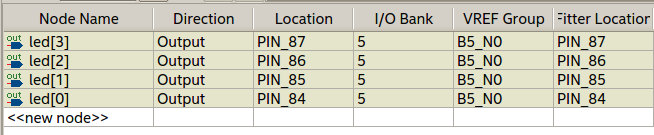
\includegraphics[scale=0.5]{images/PinPlanner_4LED.png}
\par
\caption{PIN Assignment untuk 4 LED}
\end{figure}

Compile lagi file tersebut.

Jika tidak ada pesan error, langkah selanjutnya adalah mendownload program
ini ke FPGA. Proses ini dapat dilakukan dengan cara memilih menu
\textbf{Tools -> Programmer}.
Klik button \textbf{Add File} untuk menambahkan file {\tt led\_light.sof}.
File ini biasanya ada di dalam subdirektori {\tt output} dari direktori
proyek.
Pastikan juga hardware telah terdeteksi. Jika belum terdeteksi, tambahkan melalui
dengan mengklik button \textbf{Hardware Setup}.

\begin{figure}[H]
\centering
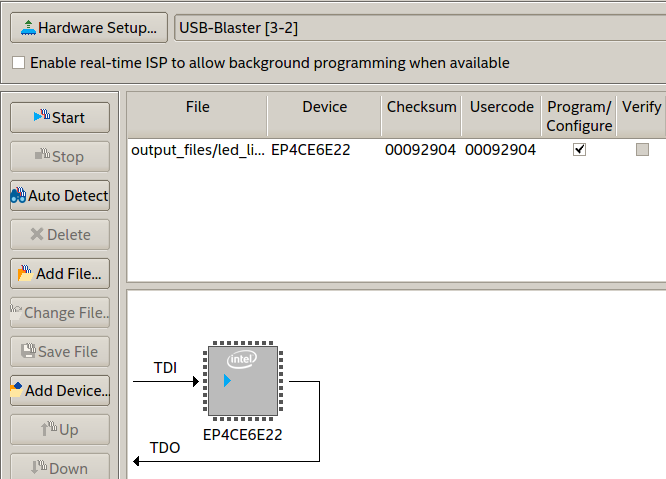
\includegraphics[scale=0.6]{images/Programmer_4LED.png}
\par
\caption{Tampilan tool \textbf{Programmer}}
\end{figure}

\begin{mdframed}[style=verilognotes,frametitle={Catatan Verilog}]
Misalkan pada board FPGA yang digunakan urutan LED dari kiri ke kanan adalah LED1,
LED2, LED3, dan LED4.

Misalkan memberikan assignment sebagai berikut.
\begin{itemize}
\item LED1 diwakili dengan {\tt led[0]}
\item LED2 diwakili dengan {\tt led[1]}
\item LED3 diwakili dengan {\tt led[2]}
\item LED4 diwakili dengan {\tt led[3]}
\end{itemize}


Misalkan juga kita memberikan nilai logika pada {\tt led} dengan
kode Verilog berikut.
\begin{verilogcode}
  led = 4'b1010;
\end{verilogcode}
Maka nilai 0 (nilai bit paling kanan atau LSB) diberikan pada {\tt led[0]}
atau LED1. Nilai pada bit kedua dari kanan diberikan untuk {\tt led[1]}, bit ketiga
untuk {\tt led[2]}, dan bit keempat (paling kiri atau MSB) untuk {\tt led[3]}.

Bagian {\tt output [3:0] led} pada kode di atas dapat diganti
dengan {\tt output [1:4] led} untuk memudahkan assignment nilai logika
sesuai dengan urutan LED di board yang digunakan. Sehingga kita dapat
melakukan assigment sebagai berikut.
\begin{itemize}
\item LED1 diwakili dengan {\tt led[1]}
\item LED2 diwakili dengan {\tt led[2]}
\item LED3 diwakili dengan {\tt led[3]}
\item LED4 diwakili dengan {\tt led[4]}
\end{itemize}

\end{mdframed}

Cobalah bereksprimen dengan cara mengganti-ganti nilai logika
dari {\tt led}, kemudian isilah tabel berikut.

\begin{table}[H]
\centering
\begin{tabular}{|c|c|}
\hline
Nilai logika & Keadaan LED (on/off) \\
\hline
0 & \\
1 & \\
\hline
\end{tabular}
\par
\end{table}


\subsubsection{Push buttons}

Buat project baru, dan buat file Verilog dengan mendefiniskan satu modul
dengan input dari push button dan output ke LED.
\begin{verilogcode}
module test_buttons( buttons, led );
  input  [3:0] buttons;
  output [3:0] led;

  assign led = buttons;
endmodule
\end{verilogcode}

Bisa juga menggunakan potongan kode berikut.
\begin{verilogcode}
  assign led[0] = buttons[0];
  assign led[1] = buttons[1];
  assign led[2] = buttons[2];
  assign led[3] = buttons[3];
\end{verilogcode}

Cobalah bereksperimen dengan kode Verilog yang ada dan juga menggukan operator Verilog
seperti 

\begin{table}[H]
\centering
\begin{tabular}{|c|c|}
\hline
Nilai logika & Keadaan PB \\
\hline
0 & \\
1 & \\
\hline
\end{tabular}
\par
\end{table}

\subsubsection{Seven segments}

Lihat Modul 1.



\subsection{Rangkaian kombinasional}

Membuat rangkaian logika digital sederhana dengan spesifikasi sebagai berikut.

\begin{itemize}
\item input push button sebanyak 3 buah, misalkan bernama {\tt A}, {\tt B}
dan {\tt C}
\item output berupa satu LED dengan nama {\tt led}
\item LED akan menyala jika jumlah push button
yang ditekan ganjil
\end{itemize}

Misalkan ketika push button ditekan nilai logikanya adalah 0 dan 
LED akan menyala jika nilai logika adalah 0, maka dapat diperoleh tabel
sebagai berikut.

\begin{table}
\centering
\begin{tabular}{|c|c|c|c|c|}
\hline
 A  &  B  &  C  & LED \\
 \hline\hline
 0  &  0  &  0  &  0  \\
 \hline
 0  &  0  &  1  &  1  \\
 \hline
 0  &  1  &  0  &  1  \\
 \hline
 0  &  1  &  1  &  0  \\
 \hline
 1  &  0  &  0  &  1  \\
 \hline
 1  &  0  &  1  &  0  \\
 \hline
 1  &  1  &  0  &  0  \\
 \hline
 1  &  1  &  1  &  1  \\
 \hline
\end{tabular}
\par
\end{table}


\begin{equation*}
LED = ABC + \bar{A}\bar{B}C + \bar{A}B\bar{C} + A\bar{B}\bar{C}
\end{equation*}

Kode Verilog yang mengimplementasikan persamaan logika di atas adalah
sebagai berikut.
\begin{verilogcode}
module deteksi_ganjil_3(
  input wire A,
  input wire B,
  input wire C,
  output wire led );

  assign led = (A & B & C) | (~A & ~B & C) | (~A & B & ~C) | (A & ~B & ~C);

endmodule
\end{verilogcode}


\subsection{BCD decoder}


\subsection{Rangkaian kombinasional}

- rangkaian pendeteksi genap ganjil, input 4 PB, output 1 LED

- Input PB -> BCD -> seven segment

- IR -> BCD -> seven segment

- Implementasi XOR

- half adder dan full adder

- Menyalakan satu atau beberapa LED dengan kombinasi input
4 push button yang diberikan.
\begin{itemize}
\item LED1 menyala jika button1 dan button3 ditekan atau button1 dan button 4 ditekan
\item LED2 menyala jika button2 dan button4 ditekan atau button1 ditekan
\end{itemize}

- Input BCD (dari ) ke output seven segment. Buat tabel kebenaran dan rangkaian (dalam skematik
atau Verilog struktural).

{\centering
\begin{tabular}{|c|c|c|c||c|c|c|c|c|c|c|c|}
\hline
\multicolumn{4}{|c||}{Input} & \multicolumn{8}{|c|}{Output} \\
\hline
PB1 & PB2 & PB3 & PB4 & a & b & c & d & e & f & g & dp \\
\hline
0 & 0 & 0 & 0 &  &  &  &  &  &  &  & \\
0 & 0 & 0 & 1 &  &  &  &  &  &  &  & \\
0 & 0 & 1 & 0 &  &  &  &  &  &  &  & \\
... & ... & ... & ... &  &  &  &  &  &  &  & \\
1 & 1 & 1 & 1 &  &  &  &  &  &  &  & \\
\hline
\end{tabular}
\par}


\subsection{Rangkaian sekuensial}

- Implementasi D flip-flop

- Implementasi J-K flip-flop dan

- Implementasi T flip-flip. Toggle operation: buzzer dan LED

- register, counter

- Kalkulator sederhana, input dari remote IR ?

- Rangkaian multiplexing LED

- Menampilkan LED perdigit


\section{Tugas Pendahuluan}


\end{document}
